
\documentclass[calculator,fluidstables,datasheet,solutions,resit]{exam}
%\documentclass[calculator,fluidstables,datasheet,resit]{exam}

% The full list of class options are
% calculator : Allows approved calculator use.
% datasheet : Adds a note that data sheet are attached to the exam.
% handbook : Allows the use of the engineering handbook.
% resit : Adds the resit markings to the paper.
% sample : Adds conspicuous SAMPLE markings to the paper
% solutions : Uses the contents of \solution commands (and \solmarks) to generate a solution file

\usepackage{pdfpages} 
\usepackage{lscape,comment}



\coursecode{EG3029}%%

\examtime{00.00--00.00}%
\examdate{00}{05}{2015}%
\examformat{Candidates must attempt \textit{all} questions.}

\newcommand{\frc}{\displaystyle\frac}
\newcommand{\br}[1]{\!\left( #1 \right)}
\newcommand{\abs}[1]{\left| #1 \right|}
\newcommand{\fracd}[2]{\frac{\mathrm{d} #1}{\mathrm{d} #2}}
\newcommand{\fracp}[2]{\frac{\partial #1}{\partial #2}}
\renewcommand{\d}[1]{\mathrm{d} #1 } 
\newcommand{\Ma}{\mathrm{M\!a}} 


\begin{document}
%%%
%%% Question 01 
%%%
\begin{question}
\begin{enumerate}[(i)]
\item Saturated refrigerant R-134a vapour at $P_{1}=400\;kPa$ is compressed by a piston to $P_{2}=16\;\text{bar}$ in a reversible adiabatic process. Critical pressure and temperature of R-134a are 4.059 MPa and 101.06$^{\text{o}}$C.
\begin{enumerate}[(a)]
\item Calculate the work done by the piston;\marks{8}
%
\solution{In order to calculate the work executed by the piston we need to calculate the thermodynamic variables at states $1$ and $2$.
\begin{enumerate}
%
\item {\bf State 1:} Saturated vapour at $P_{1}=400$ kPa = 4 bar $\Rightarrow$ $T_{1}=T_{\text{sat}}=8.93^{\text{o}}C$, $V_{1}=V_{g}=0.0509\frc{m^{3}}{kg}$, $H_{1}=252.32\frc{kJ}{kg}$, $S_{1}=0.9145\frc{kJ}{kg.K}$ and \\
${\bf U_{1}=231.97\frc{kJ}{kg}}$~\solmarks{3/8}. 
%
\item {\bf State 2:} Adiabatic (i.e., isentropic) compression to $P_{2}=16$ bar $\Rightarrow$ $S_{2}=S_{1}=0.9145\frc{kJ}{kg.K}$. At this pressure, the saturated vapour entropy is smaller than the prescribed entropy, i.e., $S_{g}=0.8982\frc{kJ}{kg.K}<<S_{2}$. Therefore, the fluid in $2$ is at superheated state, thus (via linear interpolation): $T_{2}=61.96^{\text{o}}C<<T_{C}$, $V_{2}=0.01254\frc{m^{3}}{kg}$, $H_{2}=280.77\frc{kJ}{kg}$ and \\
${\bf U_{2}=260.71\frc{kJ}{kg}}$~\solmarks{3/8}.\\
 Notice that $P_{2} << P_{C}$ and $V_{2} << V_{1}$. 
%
\end{enumerate}
 Now, from the First Law:~\solmarks{2/8}
\begin{displaymath}
dU = dQ + dW \Rightarrow U_{2}-U_{1} = 0 + \Delta W \Rightarrow {\bf \Delta W = 28.74 \frc{kJ}{kg}}
\end{displaymath}
}
%
\item Sketch the $TS$ and $PV$ diagrams including the constant pressure and temperature lines.~\marks{4}
\solution{%Figure \ref{Ex02:Q05}. ~\solmarks{4/4}
%\begin{figure}[!h]
\begin{center}~\solmarks{4/4}
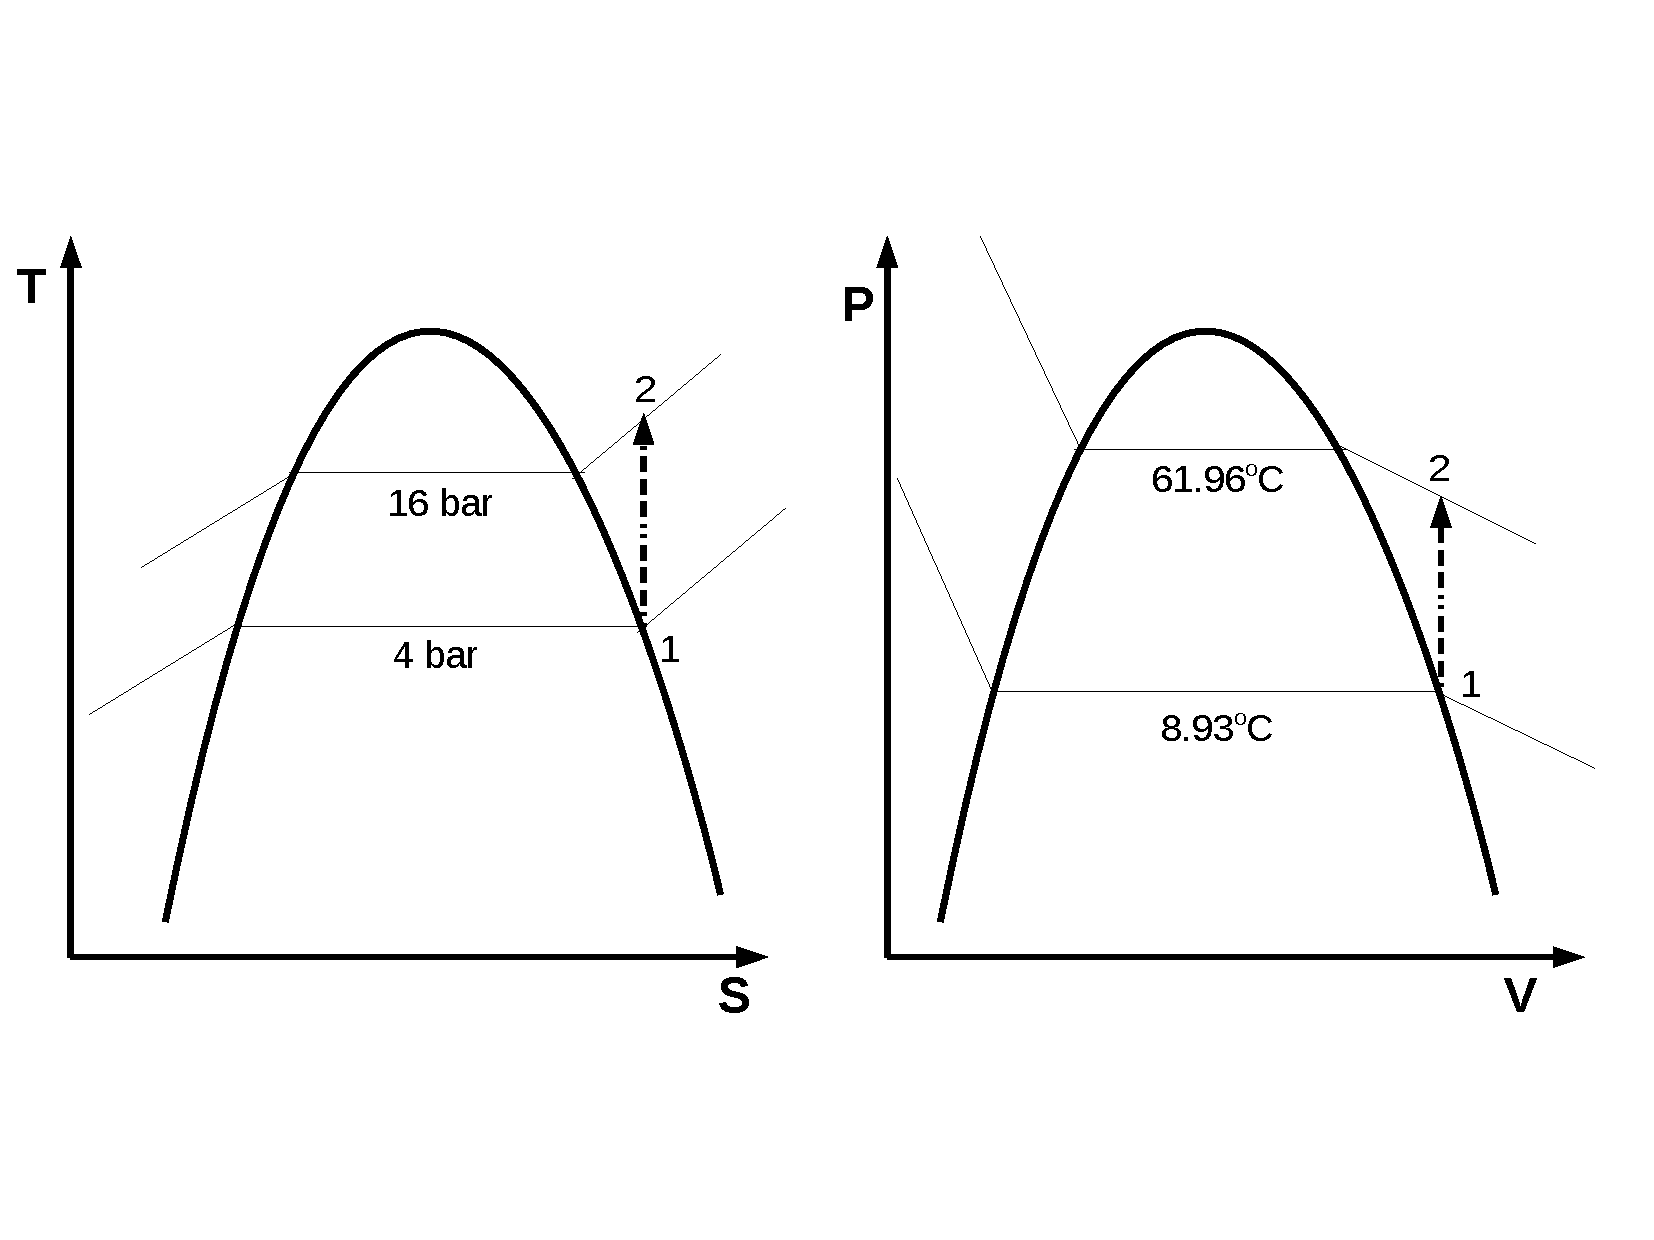
\includegraphics[width=12.0cm,height=8.0cm]{./Pics/Exam_PV-TS_Diagrams}
\end{center}
%\end{figure}
}
\end{enumerate}
%%% Saphiro 5.21 
\item A reversible power cycle receives 100 kJ by heat transfer from a hot reservoir at 327$^{\circ}$C and rejects 40 kJ by heat transfer to a cold reservoir at temperature $T_{C}$. Calculate:
\begin{enumerate}[(a)]
%
\item Thermal efficiency, $\eta_{T}\left(=\frc{W_{\text{cycle}}}{Q_{H}}\right)$, where $W_{\text{cycle}}$ is the work produced by the cycle and $Q_{H}$ is the heat associated to the hot reservoir.~\marks{4}
%
\solution{The problem supplies $Q_{H}$ = 100 kJ, $T_{H}$ = 327$^{\circ}$C and $Q_{C}$ = 40 kJ. The efficiency is given by
\begin{displaymath}
{\bf \eta_{T} } = \frc{W_{\text{cycle}}}{Q_{H}} = 1- \frc{Q_{C}}{Q_{H}} = 1 - \frc{40 kJ}{100 kJ} {\bf = 0.6} \;\; \Longrightarrow \;\; {\bf 60\%}
\end{displaymath}~\solmarks{4/4}
}  
%
\item Temperature of the cold reservoir $\left(T_{C}\right)$ in $^{\circ}$C.~\marks{4}  
%
\solution{Since the cycle operates reversibly, $\eta_{H}=\eta_{\text{max}}=1-\frc{T_{C}}{T_{H}}$. Therefore with $T_{H}$ = 327$^{\circ}$C = 600.15 K,
\begin{displaymath}
0.6 = 1 - \frc{T_{C}}{T_{H}} = 1 - \frc{T_{C}}{600.15} \;\;\Longrightarrow\;\; {\bf T_{C} = 240.06 K = -33.09^{\circ}C}
\end{displaymath}~\solmarks{4/4}
}
\end{enumerate}
%
\end{enumerate}
%
\end{question}
\clearpage

%%%
%%% Question 02
%%%
\begin{question}
\begin{enumerate}[(i)]
%
\item Derive the Maxwell relations below from the fundamental thermodynamic equations.~\marks{12}
\begin{eqnarray}
 \left(\frac{\partial T}{\partial V}\right)_{S} = -\left(\frc{\partial P}{\partial s}\right)_{V}; && 
 \left(\frc{\partial T}{\partial P}\right)_{S} = \left(\frac{\partial V}{\partial s}\right)_{P}; \nonumber \\
 \left(\frc{\partial P}{\partial T}\right)_{V} = \left(\frac{\partial S}{\partial V}\right)_{T}; &&%
  \left(\frac{\partial V}{\partial T}\right)_{P} = -\left(\frc{\partial S}{\partial P}\right)_{T} \nonumber 
\end{eqnarray}
%
\solution{First, let's assume a functional $f=f\left(a,b\right)$ and rewrite it as a function of the variables $a$ and $b$,
\begin{displaymath}
df = \left(\frc{\partial f}{\partial a}\right)_{b}da + \left(\frc{\partial f}{\partial b}\right)_{a}db
\end{displaymath}
If we define $M=\left(\frc{\partial f}{\partial a}\right)_{b}$ and $N=\left(\frc{\partial f}{\partial b}\right)_{a}$, the equation above becomes 
\begin{equation}
{\bf df = M da + N db}\label{eqn1}
\end{equation}~\solmarks{2/12}
Now, if we differentiate $M$ and $N$ with respect to $b$ and $a$, respectively,
\begin{displaymath}
\left(\frc{\partial M}{\partial b}\right)_{a} = \frc{\partial^{2} f}{\partial a\partial b}\;\;\text{ and }\;\;\left(\frc{\partial N}{\partial a}\right)_{b} = \frc{\partial^{2} f}{\partial b\partial a}
\end{displaymath}
If the functional $f$  is continuous and differentiable over all domain,
\begin{equation}\label{eqn2}
\frc{\partial^{2} f}{\partial a\partial b} = \frc{\partial^{2} f}{\partial b\partial a} \Longrightarrow {\bf \left(\frc{\partial M}{\partial b}\right)_{a} = \left(\frc{\partial N}{\partial a}\right)_{b} }
\end{equation}~\solmarks{2/12}
The fundamental thermodynamic relations, 
\begin{eqnarray}
&& dU = - PdV + TdS \nonumber \\ 
&& dH =   Tds + VdP \nonumber \\
&& dA = - PdV - SdT \nonumber \\
&& dG = - VdP - SdT \nonumber
\end{eqnarray}
have similar shape as Eqn.~\ref{eqn1}, where, for example, in the first relation: $U = f$, $M=-P$, $N=T$, $dV=da$ and $dS=db$. Using relation~\ref{eqn2}, ${\bf -\left(\frc{\partial P}{\partial S}\right)_{V}=\left(\frc{\partial T}{\partial V}\right)_{S}}$~\solmarks{2/12}. Applying the same to the remaining relations we obtain:
\begin{displaymath}
 {\bf \left(\frc{\partial T}{\partial P}\right)_{S} = \left(\frac{\partial V}{\partial s}\right)_{P}}
\end{displaymath}~\solmarks{2/12}
\begin{displaymath}
{\bf  \left(\frc{\partial P}{\partial T}\right)_{V} = \left(\frac{\partial S}{\partial V}\right)_{T}}
\end{displaymath}~\solmarks{2/12}
\begin{displaymath}
  {\bf \left(\frac{\partial V}{\partial T}\right)_{P} = -\left(\frc{\partial S}{\partial P}\right)_{T} }
\end{displaymath}~\solmarks{2/12}
}
%
\item Using the Maxwell relations above, evaluate $\left(\frc{\partial S}{\partial V}\right)_{T}$ for water vapour at 240$^{\circ}$C and specific volume of 0.4646 m$^{3}$.kg$^{-1}$ through the Redlich-Kwong equation of state,
\begin{displaymath}
P = \frc{RT}{V-b} - \frc{a}{V\left(V+b\right)T^{1/2}}
\end{displaymath}
with $a$ = 142.59 bar$\left(\frc{\text{m}^{3}}{\text{kgmol}}\right)^{2}\left(\text{K}\right)^{\frac{1}{2}}$ and $b$ = 0.0211$\frc{\text{m}^{3}}{\text{kgmol}}$.~\marks{8}
\solution{The Maxwell relation $\left(\frc{\partial P}{\partial T}\right)_{V} = \left(\frc{\partial S}{\partial V}\right)_{T}$ allows to determine $\left(\frc{\partial S}{\partial V}\right)_{T}$  from the PVT relationship in the RK EOS. Thus,
\begin{displaymath}
{\bf \left(\frc{\partial P}{\partial T}\right)_{V} = \frc{R}{V-b} + \frc{a}{2 V\left( V + b \right)T^{\frac{3}{2}}}}
\end{displaymath}~\solmarks{3/8}
Now substituting the variables by their values (and with V=0.4646 m$^{3}$.kg$^{-1}$ = 2.5811$\times$10$^{-2}$ m$^{3}$.kgmol$^{-1}$)
\begin{eqnarray}
\mathbf{\left(\frc{\partial P}{\partial T}\right)_{V}} &=& \frc{8.314\frc{kJ}{kgmol.K}}{\left(2.5811\times 10^{-2} - 0.0211\right) \frc{m^{3}}{kgmol}} + \nonumber \\
&& \frc{ 142.59\; bar\left(\frc{m^{3}}{kgmol}\right)^{2}.K^{1/2}} {2 \times 2.5811\times 10^{-2} \frc{m^{3}}{kgmol} \left( 2.5811\times 10^{-2} + 0.0211 \right) \frc{m^{3}}{kgmol} \left(513.15 K\right)^{3/2} } \nonumber  \\
&=& \mathbf{\left(\frc{\partial S}{\partial V}\right)_{T}} = \mathbf{2271.30\;\frc{kJ}{m^{3}.K}}\nonumber 
\end{eqnarray}~\solmarks{5/8}

}
%
\end{enumerate}
\end{question}
\clearpage

%%%
%%% Question 03
%%%
\begin{question}
The steam generator of a nuclear power plant produces 25 kg.s$^{-1}$ of water-steam at P$_{1}$ = 140 bar and T$_{1}$= 415$^{\circ}$C. The fluid is used to drive a turbine (isentropic expansion) producing power $\left(W_{T}\right)$ at P$_{2}$ = 2.5 bar. Before the vaporisation in the boiler, the fluid needs to be condensed into liquid water (stage 3) producing $Q_{C}$ of heat. 
\begin{center}
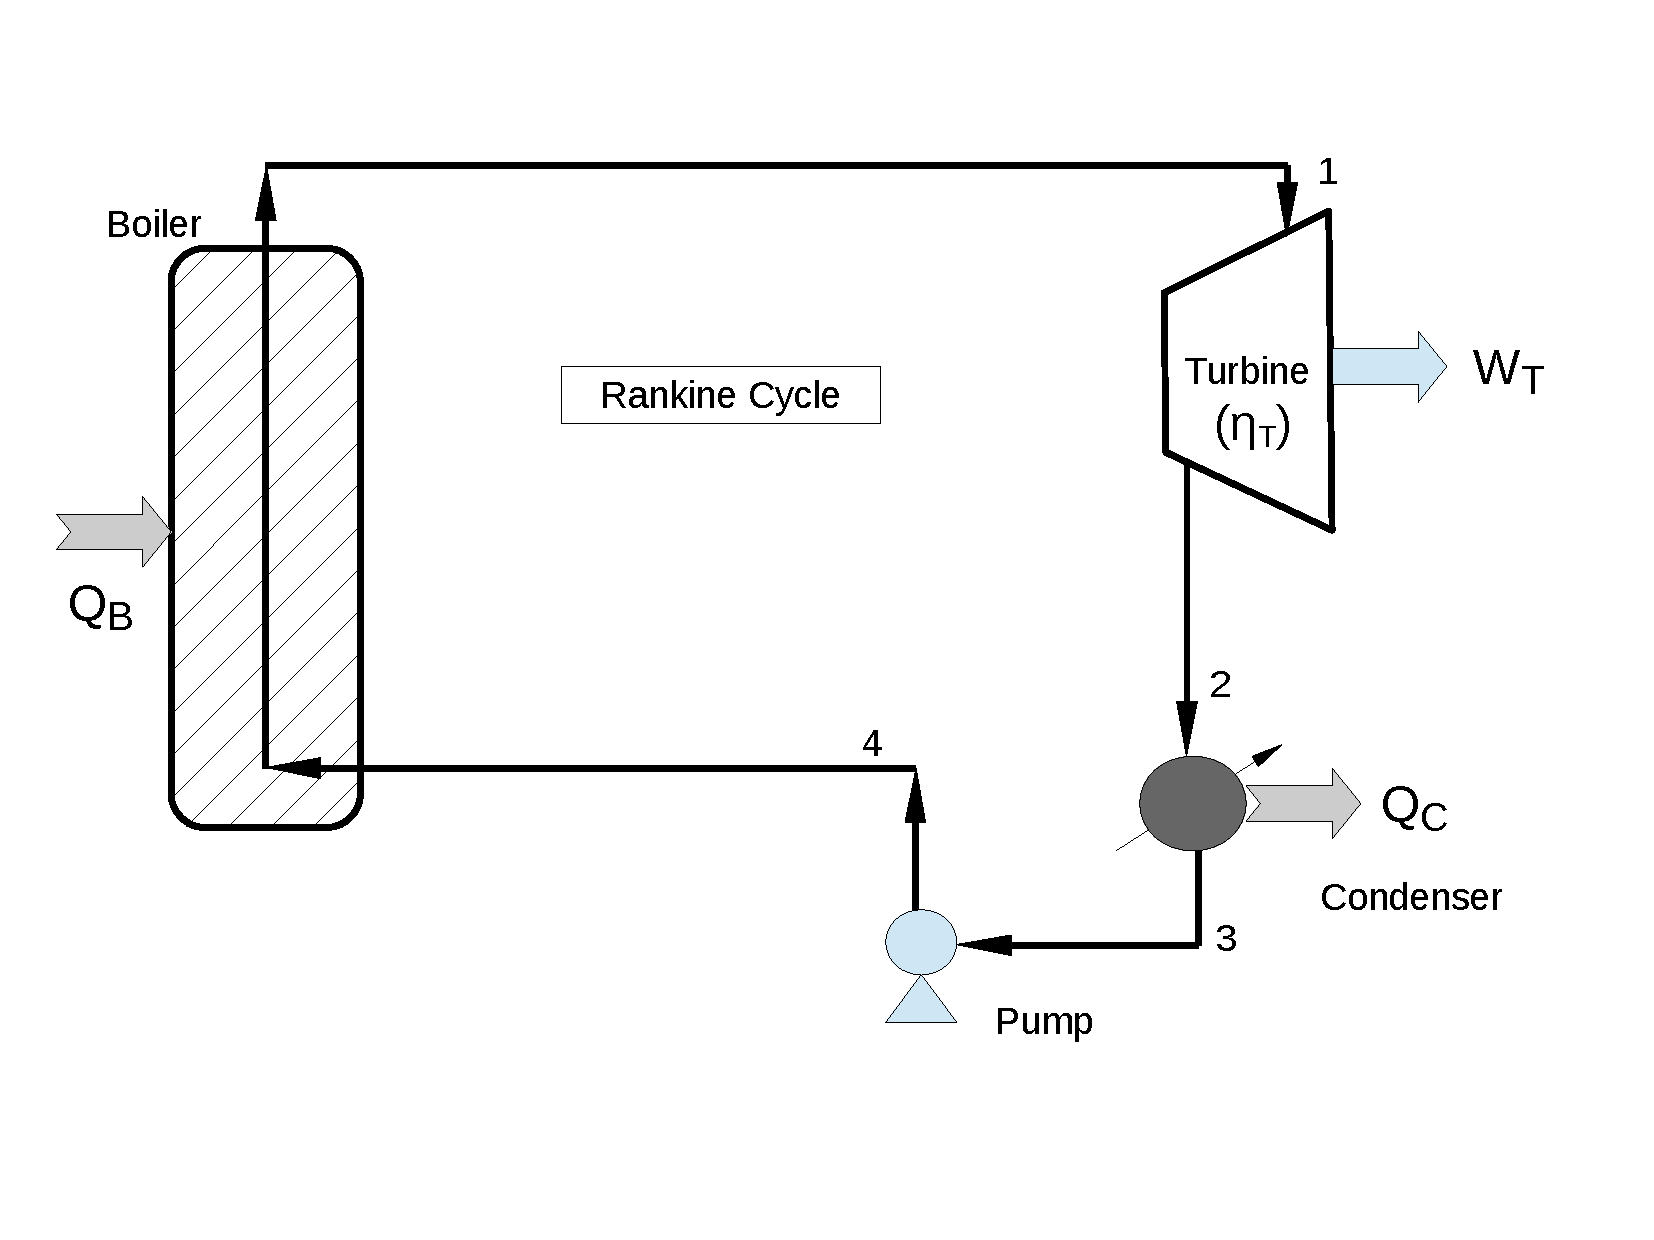
\includegraphics[width=10.cm,height=8.cm,clip]{./Pics/RankineCycle2}
%\caption{ Reheat and regenerative Rankine cycle with 2 turbines.}
\label{exam_mod02_rankinecycle}
\end{center}
\begin{enumerate}[(a)]
\item Calculate $H_{1}, H_{2}, H_{4}, S_{1} \text{ and } x_{2}$ (quality of the steam).~\marks{10}
%
\solution{\begin{description}
\item[State 1:] At P$_{1}$ = 140 bar, T$_{sat}$ = 336.75$^{\circ}$C $>$ T$_{1}$= 415$^{\circ}$C, therefore the fluid is at superheated state. From the superheated steam table (via linear interpolation), {\bf H$_{1}$ = 3054.51 kJ.kg$^{-1}$}~\solmarks{2/10} and \\
{\bf S$_{1}$ = 6.0208 kJ.(kg.K)$^{-1}$}~\solmarks{2/10}.
\item[State 2:] Isentropic expansion at P$_{2}$ = 2.5 bar $\longrightarrow$ S$_{2}$=S$_{1}$. We can calculate the quality of the water-steam at 2.5 bar,
\begin{displaymath}
{\bf x_{2}} = \frc{S_{2}-S_{f}}{S_{g}-S_{f}} {\bf = 0.8105} 
\end{displaymath}~\solmarks{2/10}
With the quality we can then calculate the H$_{2}$,
\begin{displaymath}
x_{2} = \frc{H_{2}-H_{f}}{H_{g}-H_{f}} \;\;\Longrightarrow \;\; {\bf H_{2} = 2303.50\frc{kJ}{kg}} 
\end{displaymath}~\solmarks{2/10}
\item[State 3:] After the condenser, water is at liquid state at P$_{3}$=P$_{2}$ (no pressure drop) with H$_{3}$ = H$_{f}$ = 535.37 kJ.kg$^{-1}$, S$_{3}$ = S$_{f}$ = 1.6072 kJ.(kg.K)$^{-1}$ and V$_{3}$ = V$_{f}$ = 1.0672$\times$10$^{-3}$ m$^{3}$.kg$^{-1}$.
\item[State 4:] Assuming the liquid water is incompressible $dH\equiv VdP$ with P$_{4}$ = P$_{1}$
\begin{displaymath}
{\bf H_{4}} = H_{3} + V_{3}\left(P_{4} - P_{3}\right) = {\bf 550.04 \frc{kJ}{kg}}
\end{displaymath}~\solmarks{2/10}
\end{description}
}
%
\item Determine the power produced in the turbine $\left(W_{T}\right)$ in MW.~\marks{2}
%
\solution{For $\dot{m}_{w}$ = 25 kg.s$^{-1}$,
\begin{displaymath}
{\bf W_{T}} = \dot{m}_{w}\left(H_{1}-H_{2}\right) {\bf = 18775.25\frc{kJ}{s} = 18.8 MW}
\end{displaymath}~\solmarks{2/2}
}
%
\item Determine the heat extracted from the steam $\left(Q_{C}\right)$ in MW.~\marks{2}
%
\solution{\begin{displaymath}
{\bf Q_{C} }= \dot{m}_{w}\left(H_{2}-H_{3}\right) {\bf = 44203.25\frc{kJ}{s} = 44.2 MW}
\end{displaymath}~\solmarks{2/2}
}
\item Determine the heat supplied by the boiler $\left(Q_{B}\right)$ in MW.~\marks{2}
%
\solution{\begin{displaymath} 
{\bf Q_{B}} = \dot{m}_{w}\left(H_{1}-H_{4}\right) {\bf = 62611.75\frc{kJ}{s} = 62.6 MW}
\end{displaymath}~\solmarks{2/2}
}
%
\item Calculate the efficiency of the cycle $\left(\eta_{\text{cycle}}=\frac{W_{T}}{Q_{B}}\right)$.~\marks{2}
%
\solution{\begin{displaymath}
{\bf \eta_{\text{cycle}} } =  \frc{W_{T}}{Q_{B}} {\bf = 0.30} \Longrightarrow {\bf 30\%}
\end{displaymath}~\solmarks{2/2}
}
%
\item Sketch the temperature $\times$ entropy (TS) diagram for the process indicating the liquid and vapour saturated lines and each stage of the water-steam Rankine cycle.~\marks{2}
\solution{~\solmarks{2/2}
\begin{center}
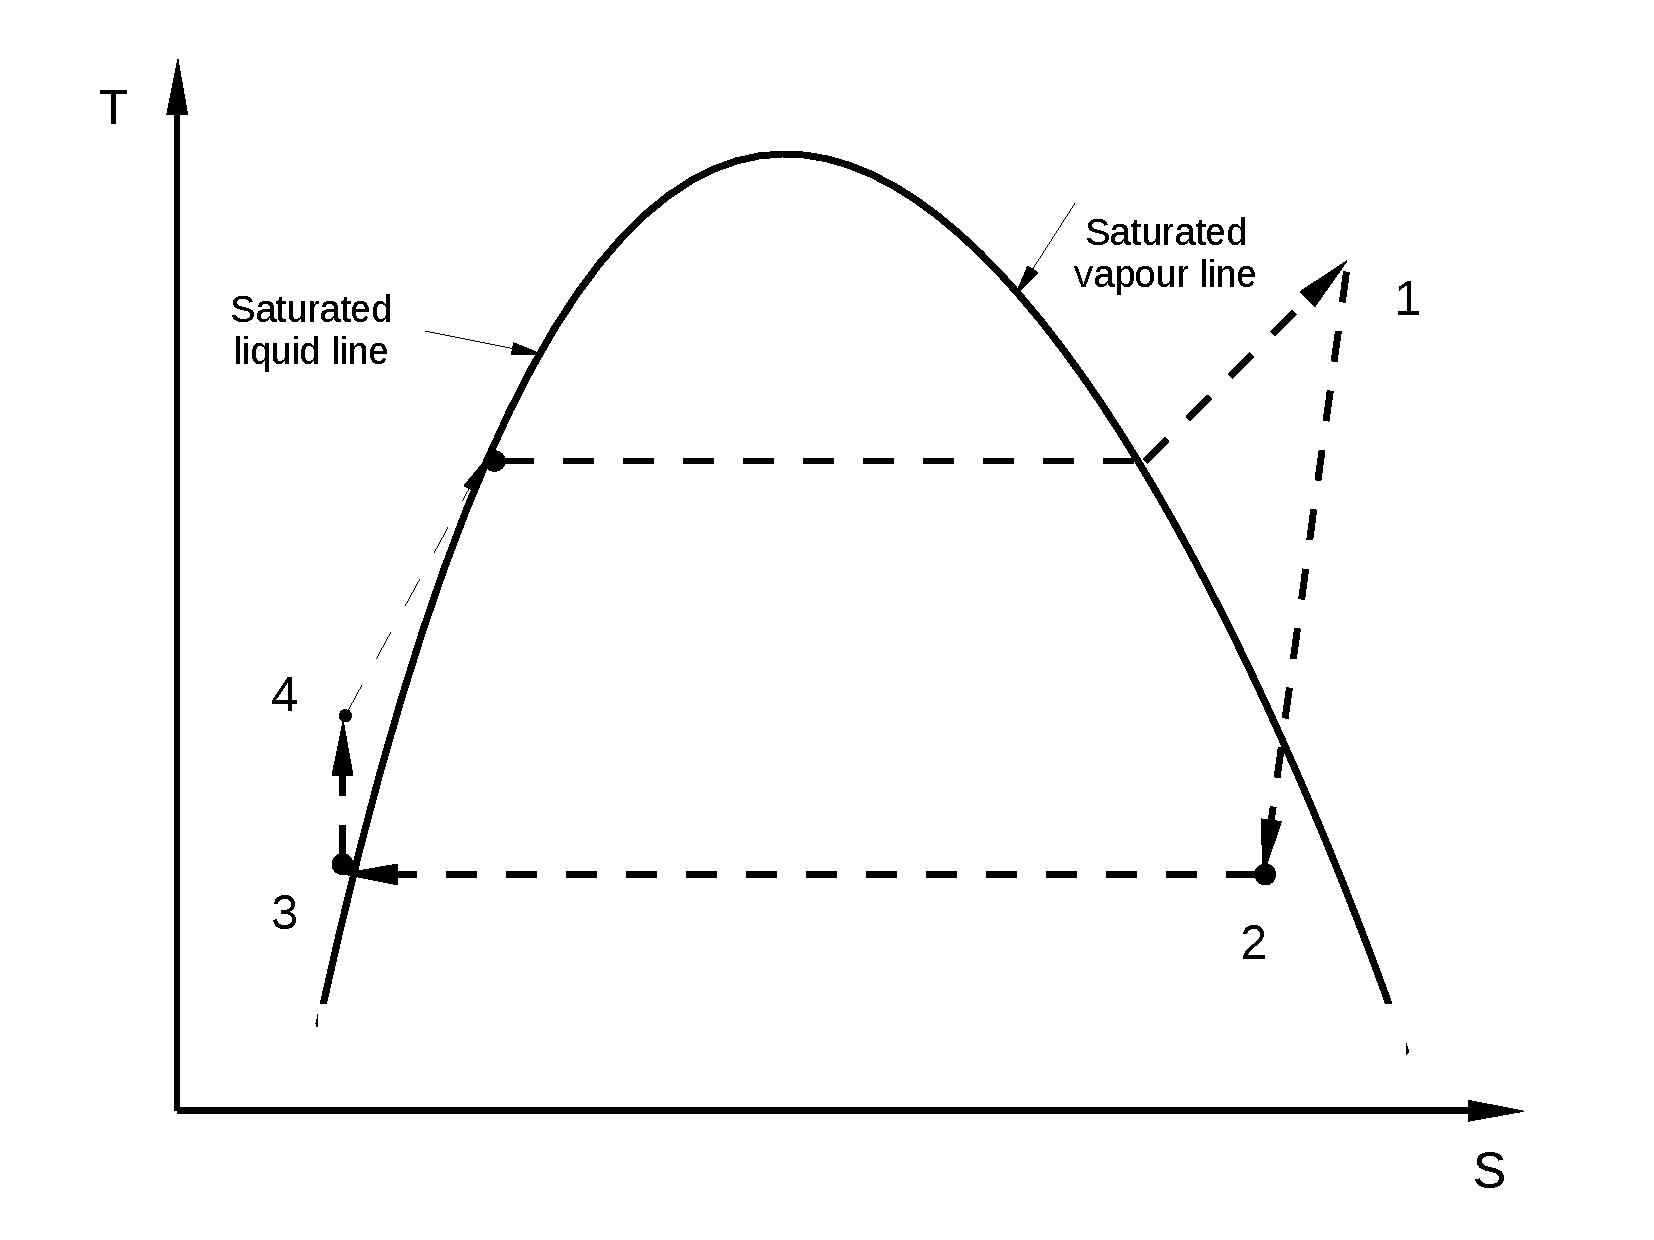
\includegraphics[width=8.cm,clip]{./Pics/TS_DIagramExam2}
\end{center}%~\solmarks{3/3}
}
\end{enumerate}
To solve this problem, you should assume that the saturated liquid streams are incompressible, and therefore $dH = VdP$ (where $H$, $V$ and $P$ are enthalpy, volume and pressure, respectively). Quality of the vapour is expressed as
\begin{displaymath}
x_{j} = \frc{\Psi_{j}-\Psi_{f}}{\Psi_{g}-\Psi_{f}}\;\;\;\text{with }\Psi=\left\{H,S\right\}
\end{displaymath}
where $S$ is the entropy. 

\end{question}
\clearpage

%%%
%%% QUESTION 4 (SM&VN 12.26)
%%%
\begin{question}
Two chemical species, $1$ and $2$ are mixed in a solution at 25$^{\circ}$C and atmospheric pressure. The volume change is given by the following equation,
\begin{displaymath}
\Delta V = x_{1}x_{2}\left(45 x_{1} +  25x_{2}\right)
\end{displaymath} 
where $\Delta V$ is expressed in cm$^{3}$.gmol$^{-1}$. At these temperature and pressure conditions, V$_{1}$ = 110 and V$_{2}$ = 90 cm$^{3}$.gmol$^{-1}$. Determine the partial molar volumes of the chemical species in a solution containing 40$\%$-mol of species $1$.~\marks{20}
\solution{ $x_{1} = 0.4$ and $x_{2}=1-x_{1}=0.6$.  The volume change is the excess volume,
\begin{displaymath}
\Delta V = x_{1}x_{2}\left(45 x_{1} +  25x_{2}\right) = {\bf V^{\text{E}} = 7.92\frc{cm^{3}}{gmol}}
\end{displaymath}~\solmarks{5/20}
The volume of the binary solution is given by
\begin{displaymath}
{\bf V} = V^{\text{E}} + x_{1}V_{1}+x_{2}V_{2} {\bf = 105.92 \frc{cm^{3}}{gmol}}
\end{displaymath}~\solmarks{5/20}
The partial molar properties in binary mixtures can be obtained by $\overline{M}_{1} = M + x_{2}\frc{d M}{dx_{1}}$ and $\overline{M}_{2} = M - x_{1}\frc{d M}{dx_{1}}$, thus for partial molar volumes
\begin{displaymath}
{\bf \overline{V}_{1}} = V + x_{2} \frc{d V}{dx_{1}} {\bf = 124.76 \frc{cm^{3}}{gmol}}
\end{displaymath}~\solmarks{3/20}
and
\begin{displaymath}
  {\bf \overline{V}_{2}} = V - x_{1} \frc{d V}{dx_{1}} {\bf = 93.36 \frc{cm^{3}}{gmol}}
\end{displaymath}~\solmarks{3/20}
where
\begin{eqnarray}
V &=& V^{\text{E}} + \sum\limits_{i=1}^{n}x_{i}V_{i}  = x_{1}x_{2}\left(45x_{1}+25x_{2}\right)+x_{1}V_{1}+x_{2}V_{2}  \nonumber \\
  &=&  x_{1}\left(1-x_{1}\right)\left[45x_{1}+25\left(1-x_{1}\right)\right]+x_{1}V_{1}+\left(1-x_{1}\right)V_{2} \nonumber
\end{eqnarray}
and
\begin{displaymath}
\mathbf{\frc{dV}{dx_{1}} = 25 -10x_{1}-60x_{1}^{2} + \left(V_{1}-V_{2}\right)}
\end{displaymath}~\solmarks{4/20}

We can verify the solution through
\begin{displaymath}
V = x_{1}\overline{V}_{1}+x_{2}\overline{V}_{2}=105.92 \frc{cm^{3}}{gmol}
\end{displaymath}
}
\end{question}

\clearpage

%%%
%%% QUESTION 5
%%%
\begin{question}
\begin{enumerate}[(i)]
% SM&VN 10.13
\item A concentrated binary solution containing mainly species $2$ $\left(\text{though } x_{2}\not= 1\right)$ is in equilibrium with a vapour phase containing both species $1$ and $2$. Pressure and temperature of this two-phase system are 1 bar and 298.15 K. Given $\mathcal{H}_{1}$ = 200 bar (Henry constant) and P$_{2}^{\text{sat}}$ = 0.10 bar, calculate $x_{1}$ and $y_{1}$.~\marks{10/10}
%
\solution{Assuming that at 1 bar the vapour phase behaves as an ideal gas. The vapour phases fugacities are then equal to the partial pressures. Assume the Lewis/Randall rule applies to concentrated species $2$ and that Henry's law applies to dilute species $1$, therefore,
\begin{displaymath}
y_{1}P=\mathcal{H}_{1}x_{1};\;\;\text{ and }\;\; y_{2}P= x_{2}P_{2}^{\text{sat}}
\end{displaymath}
with $x_{1}+x_{2}=1$. Thus $P = y_{1}P + y_{2}P$ becomes,~\solmarks{5/10}
\begin{displaymath}
P = \mathcal{H}_{1}x_{1}+\left(1-x_{1}\right)P_{2}^{\text{sat}} \;\;\Longrightarrow {\bf x_{1} = 4.502\times 10^{-3}}
\end{displaymath}
and ${\bf y_{1}=\frc{\mathcal{H}_{1}x_{1}}{P}=0.9}$.~\solmarks{5/10}
}
%
% SM&VN 10.19
\item Chemical species $A$ and $B$ are in vapour-liquid equilibrium at 298.15 K. The following conditions are applied to this system:\begin{center}
\begin{tabular}{l l}
$\ln\gamma_{A} = 1.8x_{B}^{2}$ & $\ln\gamma_{B}=1.8x_{A}^{2}$ \\
$P_{A}^{\text{sat}}$ = 1.24 bar & $P_{B}^{\text{sat}}$ = 0.89 bar
\end{tabular} 
\end{center}
Assuming that $y_{i}P = x_{i}\gamma_{i}P_{i}^{\text{sat}}$ (where $\gamma_{i}$ is the activity coefficient of species $i$) is valid, 
\begin{enumerate}[(a)]
\item Calculate the pressure $P$ and the vapour mole fraction $y_{A}$ for a liquid mole fraction $x_{A}=0.65$.~\marks{6}
%
\solution{With $x_{A}$ =0.65 and $x_{B}$=0.35, we can calculate the activity coefficients, $\gamma_{A}$ $\gamma_{B}$ and apply in $P = x_{A}\gamma_{A} P_{A}^{\text{sat}} + x_{B}\gamma_{B} P_{B}^{\text{sat}}$ leading to {\bf P=1.671 bar}~\solmarks{3/6}. The vapour mole fraction is obtained from $y_{A} = \frc{x_{A}\gamma_{A}P_{A}^{\text{sat}}}{P}$, leading to  ${\bf y_{A}=0.6013}$.~\solmarks{3/6} 
} 
%
\item Calculate the range of overall mole fraction $z_{A}$ in which this system may exist.~\marks{4}
\solution{From mass balance for species $A$~\solmarks{1/4}
\begin{displaymath}
z_{A} = V y_{A} + L x_{A} \Longrightarrow z_{A} =V y_{A} + (1-V)x_{A} \Longrightarrow {\bf V= \frc{z_{A}-x_{A}}{y_{A}-x_{A}}}
\end{displaymath}
The overall vapour mole fraction $V$, varies from 0 to 1, ${\bf 0\leq V\leq 1}$~\solmarks{1/4}, therefore (replacing in the equation above) ${\bf 0.6013\leq z_{A} \leq 0.65}$.~\solmarks{2/4}
}
\end{enumerate}

\end{enumerate}

\end{question}


\clearpage
\begin{itemize}
%%%
\item Generic cubic equation of state:
\begin{eqnarray}
&& Z= 1 + \beta - q\beta \frc{Z - \beta} {\left(Z+\varepsilon\beta\right)\left(Z+\sigma\beta\right)}  \;\;\text{(vapour and vapour-like roots)}\nonumber\\
&& Z= 1 + \beta + \left(Z + \epsilon\beta\right)\left(Z+\sigma\beta\right)\left(\frc{1+\beta-Z}{q\beta}\right)  \;\;\text{(liquid and liquid-like roots)}\nonumber\\
&& \text{with }\; \beta=\Omega\frc{P_{r}}{T_{r}} \;\;\text{ and } \;\; q=\frc{\Psi\alpha\left(T_{r}\right)}{\Omega T_{r}}  \nonumber \\
&&\alpha_{\text{SRK}} = \left[ 1 + \left( 0.480 + 1.574 \omega - 0.176\omega^{2}\right)\left(1-\sqrt{T_{r}}\right)\right]^{2}  \nonumber \\
&&\alpha_{\text{PR}} = \left[ 1 + \left( 0.37464 + 1.54226 \omega - 0.26992\omega^{2}\right)\left(1-\sqrt{T_{r}}\right)\right]^{2} \nonumber
\end{eqnarray} 
    \begin{center}
       \begin{tabular}{| l | c c c c c| }
       \hline
          {\bf EOS}  & {\bf $\alpha$} & {\bf $\sigma$}  & {\bf $\varepsilon$} & {\bf $\Omega$} & {\bf $\Psi$ } \\
       \hline
            vdW      & 1              & 0               & 0                  & 1/8            & 27/64          \\
            RK       & T$_{r}^{-1/2}$  & 1                & 0                  & 0.08664       & 0.42748        \\
           SRK       &$\alpha_{\text{SRK}}$& 1            & 0                   & 0.08664       & 0.42748        \\
            PR       &$\alpha_{\text{PR}}$& 1+$\sqrt{2}$   & 1-$\sqrt{2}$        & 0.07780        & 0.45724  \\
       \hline
       \end{tabular}
    \end{center}

%%%
\item Newton-Raphson (root-finder) method: $X_{i} = X_{i-1} - \frc{\mathcal{F}\left(X_{i-1}\right)}{d\mathcal{F}/dX\left(X_{i-1}\right)}$

%%%
\item Fundamental thermodynamic equations:\\
\begin{tabular}{c c c c}
$dU = dQ + dW$;  & $dH = dU + d(PV)$; & $dA = dU -d(TS)$; & $dG=dH-d(TS)$ \\
$dU = TdS - PdV$;& $dH = TdS + VdP$;  & $dA = -SdT - PdV$;& $dG = -SdT + VdP$ \\ 
\end{tabular}\\
\begin{tabular} {c c}
$dH = C_{p}dT + \left[ V - T\left(\frc{\partial V}{\partial T}\right)_{P}\right]dP$; &  $dS=C_{p}\frc{dT}{T} - \left(\frc{\partial V}{\partial T}\right)_{P}dP$ \\
$dU = C_{v}dT + \left[T\left(\frc{\partial P}{\partial T}\right)_{V} - P\right]dV$;  & $dS = C_{v}\frc{dT}{T} - \left(\frc{\partial P}{\partial T}\right)_{V}dV$
\end{tabular}

%%% 
\item Polytropic Relations:\\
\begin{displaymath} 
\frc{T_{2}}{T_{1}} =\left(\frc{P_{2}}{P_{1}}\right)^{\frac{\gamma-1}{\gamma}} = \left(\frc{V_{1}}{V_{2}}\right)^{\gamma-1}\;\; ; 
TV^{\gamma-1} =\text{ const};\; TP^{\frac{1-\gamma}{\gamma}}=\text{ const};\; PV^{\gamma}=\text{ const} 
\end{displaymath}

%%%
\item Raoult's Law:\\
\begin{displaymath}
y_{i}P = x_{i}P_{i}^{\text{sat}}\;\;\;\text{ and } \;\;\; y_{i}P = x_{i}\gamma_{i}P_{i}^{\text{sat}}\;\;\;\text{ with } i=1,2,\cdots N
\end{displaymath}

%%%
\item Henry's Law:\\
\begin{displaymath}
x_{i}\mathcal{H}_{i} = y_{i}P\;\;\;\text{ with } i=1,2,\cdots N
\end{displaymath}

%%%
\item Antoine Equation:\\
\begin{displaymath}
\log_{10} P^{\star} = A-\frc{B}{T+C}\;\;\;\text{ with P}^{\star}\text{ in mm-Hg and T in }^{\circ}\text{C}
\end{displaymath}

%%%
\item Solutions:\\
\begin{displaymath}
M^{\text{E}} = M - \sum\limits_{i=1}^{N} x_{i}M_{i}; \; \overline{M}_{1}=M+x_{2}\frc{d M}{dx_{1}};\; \overline{M}_{2} = M - x_{1}\frc{d M}{dx_{1}}
\end{displaymath}

\end{itemize}

%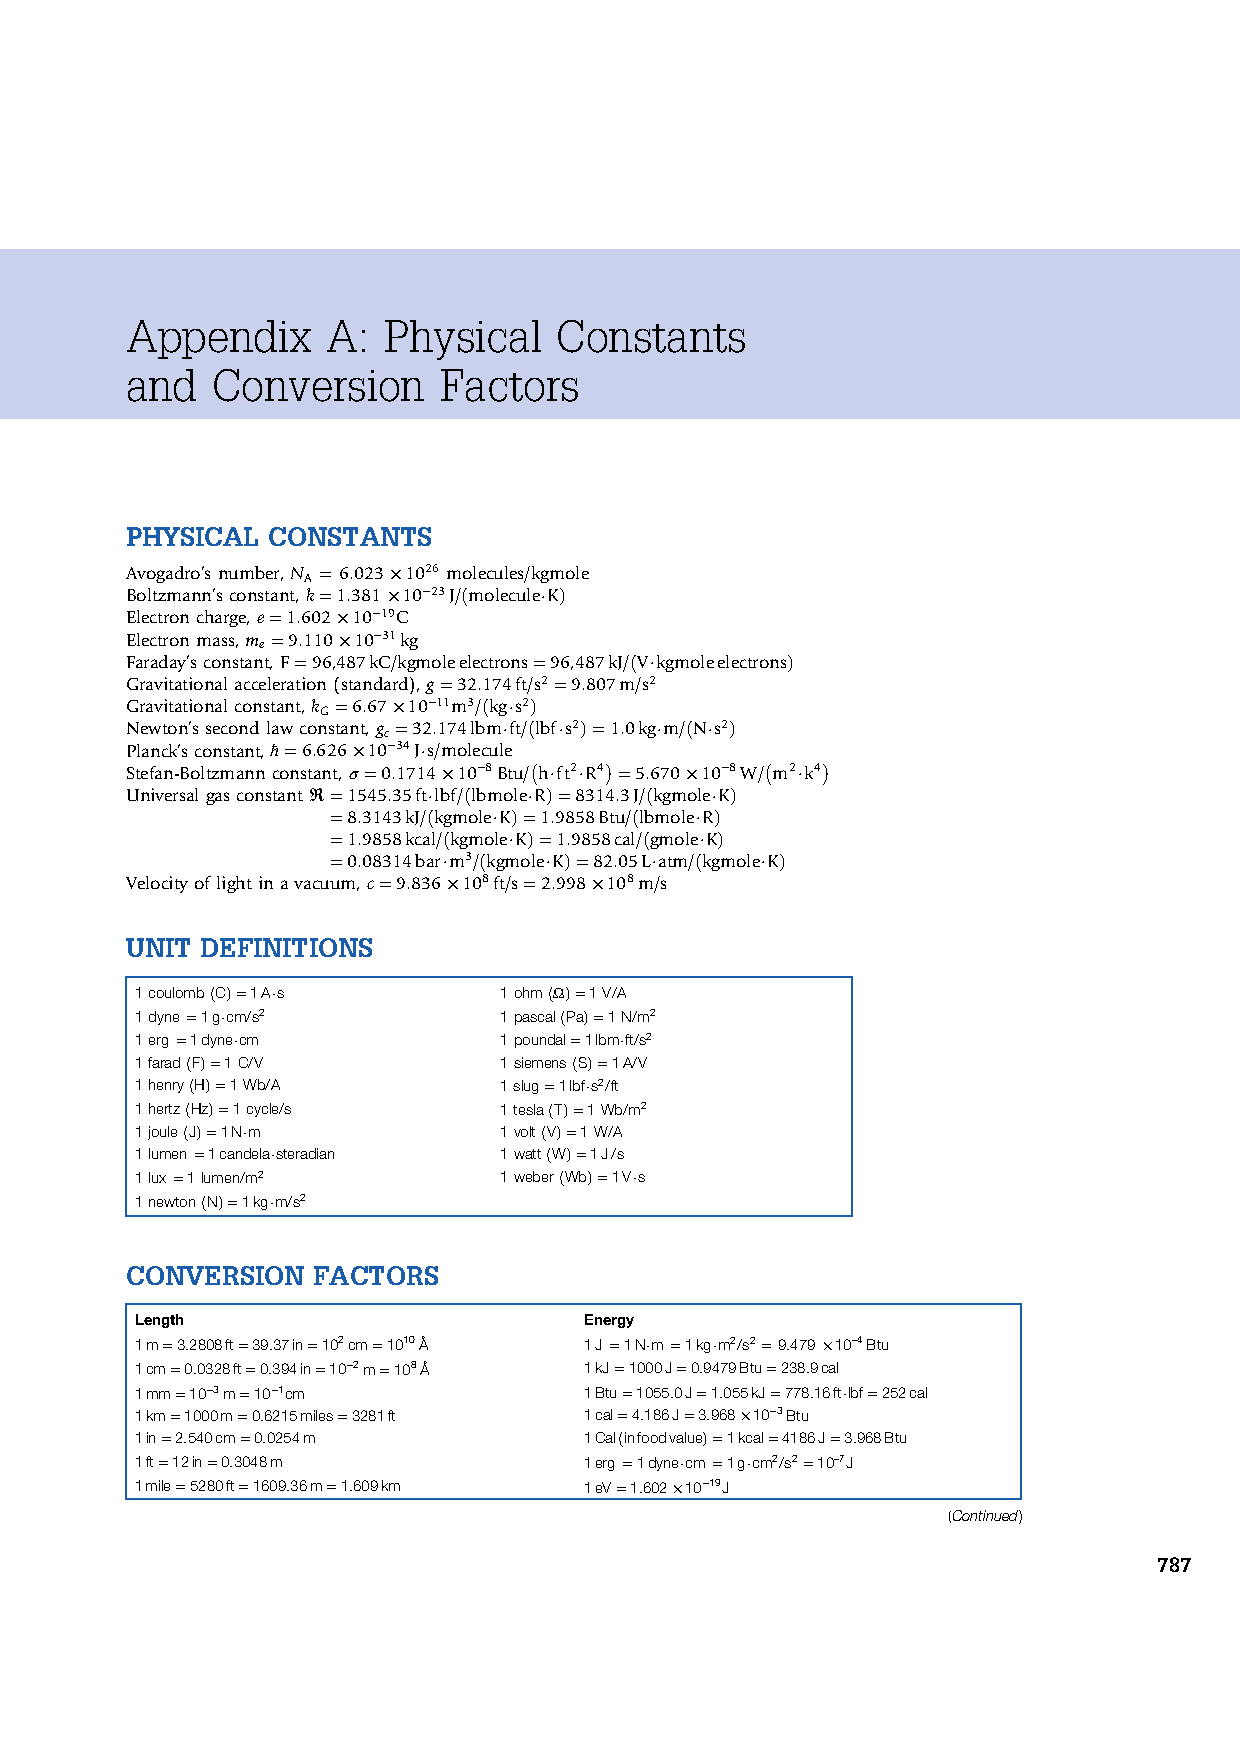
\includepdf[pages={1-10}]{./Pics/Water_R134_UnitConv}

\clearpage
\end{document}
